\documentclass[12pt]{article}

\usepackage[margin=1in]{geometry}
\usepackage{graphicx}
\usepackage{newtxtext,newtxmath}  % Times New Roman text + math (APA)
\usepackage{setspace}
\usepackage{microtype}
\usepackage[hidelinks]{hyperref}
\usepackage{enumitem}

\setlength{\parindent}{0pt}
\setlength{\parskip}{6pt}

\title{Appendix B: Individual-Participant Model Fits}
\author{}
\date{}

\begin{document}

\maketitle
\vspace{-2.5em}

The figures below show trial-by-trial model fits for a random, group-balanced
subset of 8 participants (4 from each group), drawn
with a fixed seed for reproducibility from those with at least 15
recorded choices and no exclusive preference for a single alternative in each
condition (the Piranha condition is exempt in the 5:1 group, where it typically
ends before 15 choices accrue). Whereas the
figures in the main text
aggregate across participants, every model in this paper was fit at the
participant level; these panels illustrate the per-participant fits that
underlie those group summaries. Each figure is a $2\times2$ grid, one panel per
earning-budget condition. Black x marks show the participant's raw choice on
each trial (smaller--sooner ${}=1$, larger--later ${}=0$), plotted just
outside the $[0,1]$ band so they do not overlap the model lines. The gray lines
are the predicted probability of choosing the smaller--sooner option,
$P(\mathrm{SS})$,
from the best-performing model in each of the six families (lowest median
corrected Akaike information criterion at the pooled fit scope):

\begin{itemize}[noitemsep,topsep=0pt]
  \item \textbf{baseline}: Logistic
  \item \textbf{energy\_budget}: Marginal Value (Fitted ρ)
  \item \textbf{historical\_dynamics}: Ratio Invariance
  \item \textbf{rl\_action\_value}: Q-Learning (Condition-Aware)
  \item \textbf{rl\_state\_action}: Q-Table (Operant State)
  \item \textbf{human\_as\_qtable}: Human-as-Q-Table (Operant State)
\end{itemize}

\clearpage

\begin{figure}[p]
  \centering
  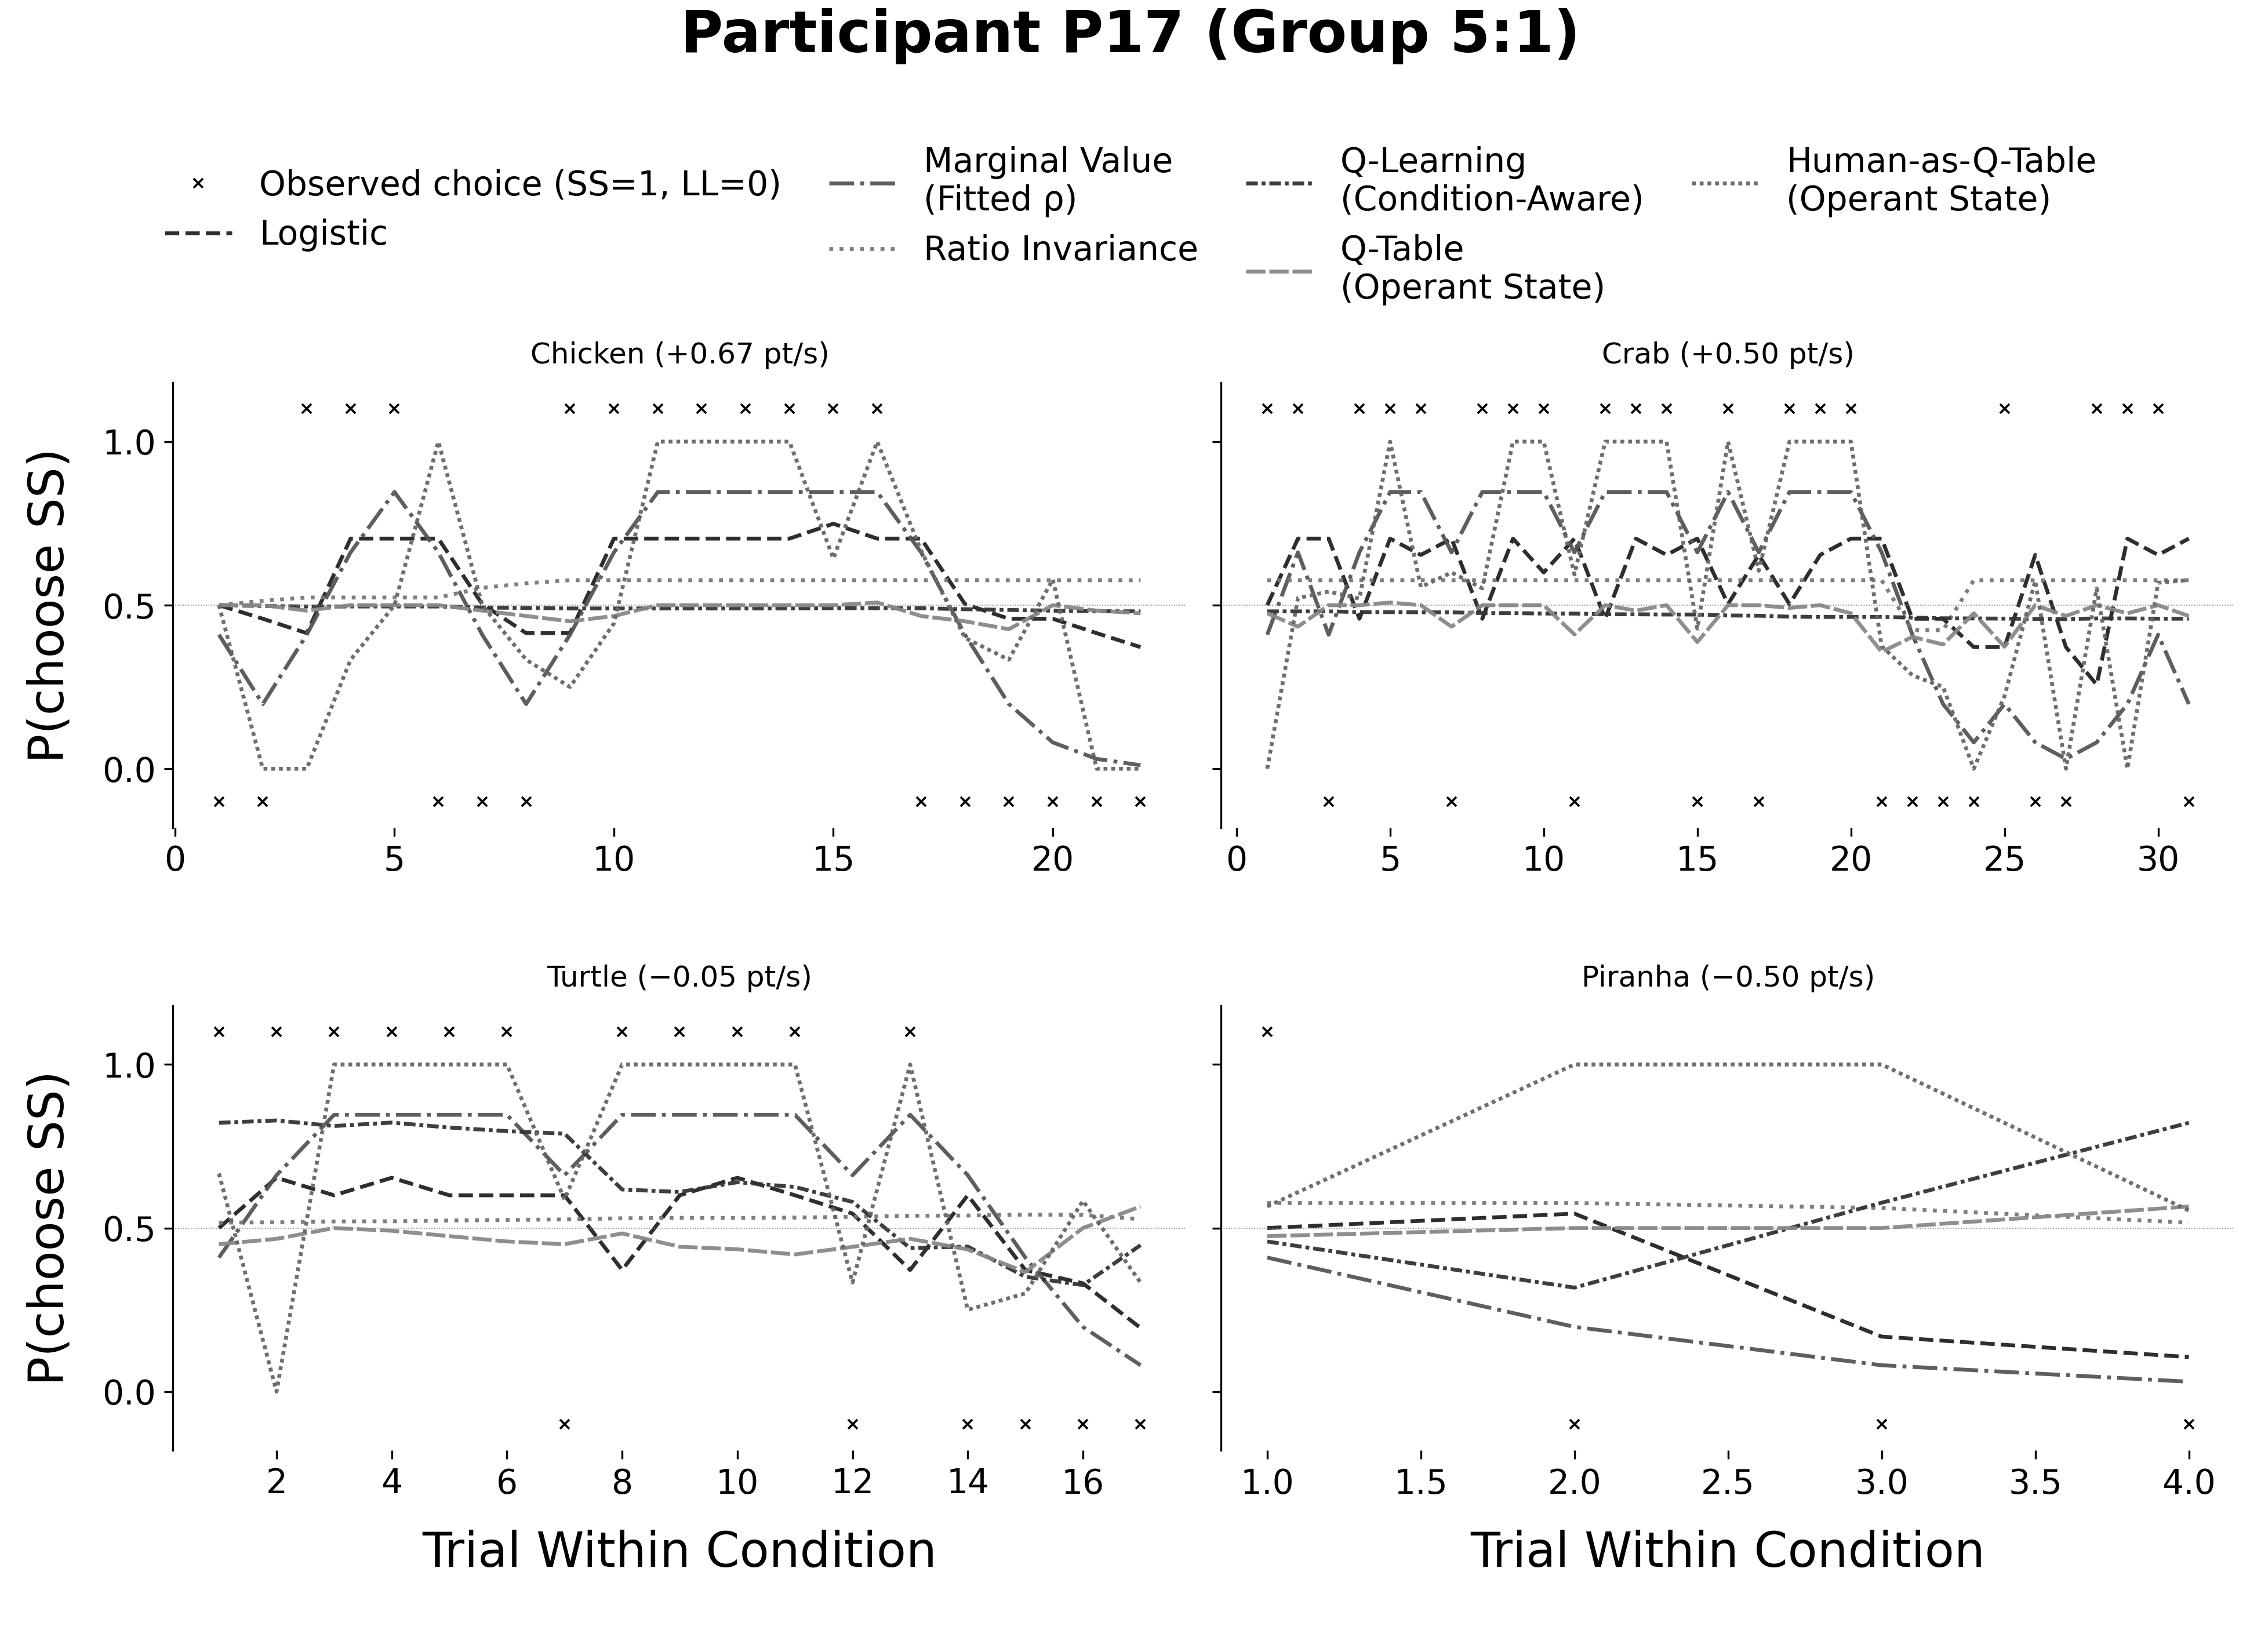
\includegraphics[width=\textwidth]{data/results/figures/appendix_b/fig_participant_Exp1_05_P17.png}
  \caption{Trial-by-trial model fit for participant Exp1\_05\_P17 (Group 5:1). Each panel is one earning-budget condition. Black x marks are the participant's raw choices (SS${}=1$, LL${}=0$), plotted just outside the $[0,1]$ band. Gray lines are the predicted $P(\mathrm{SS})$ of the best-fitting model in each family.}
\end{figure}

\begin{figure}[p]
  \centering
  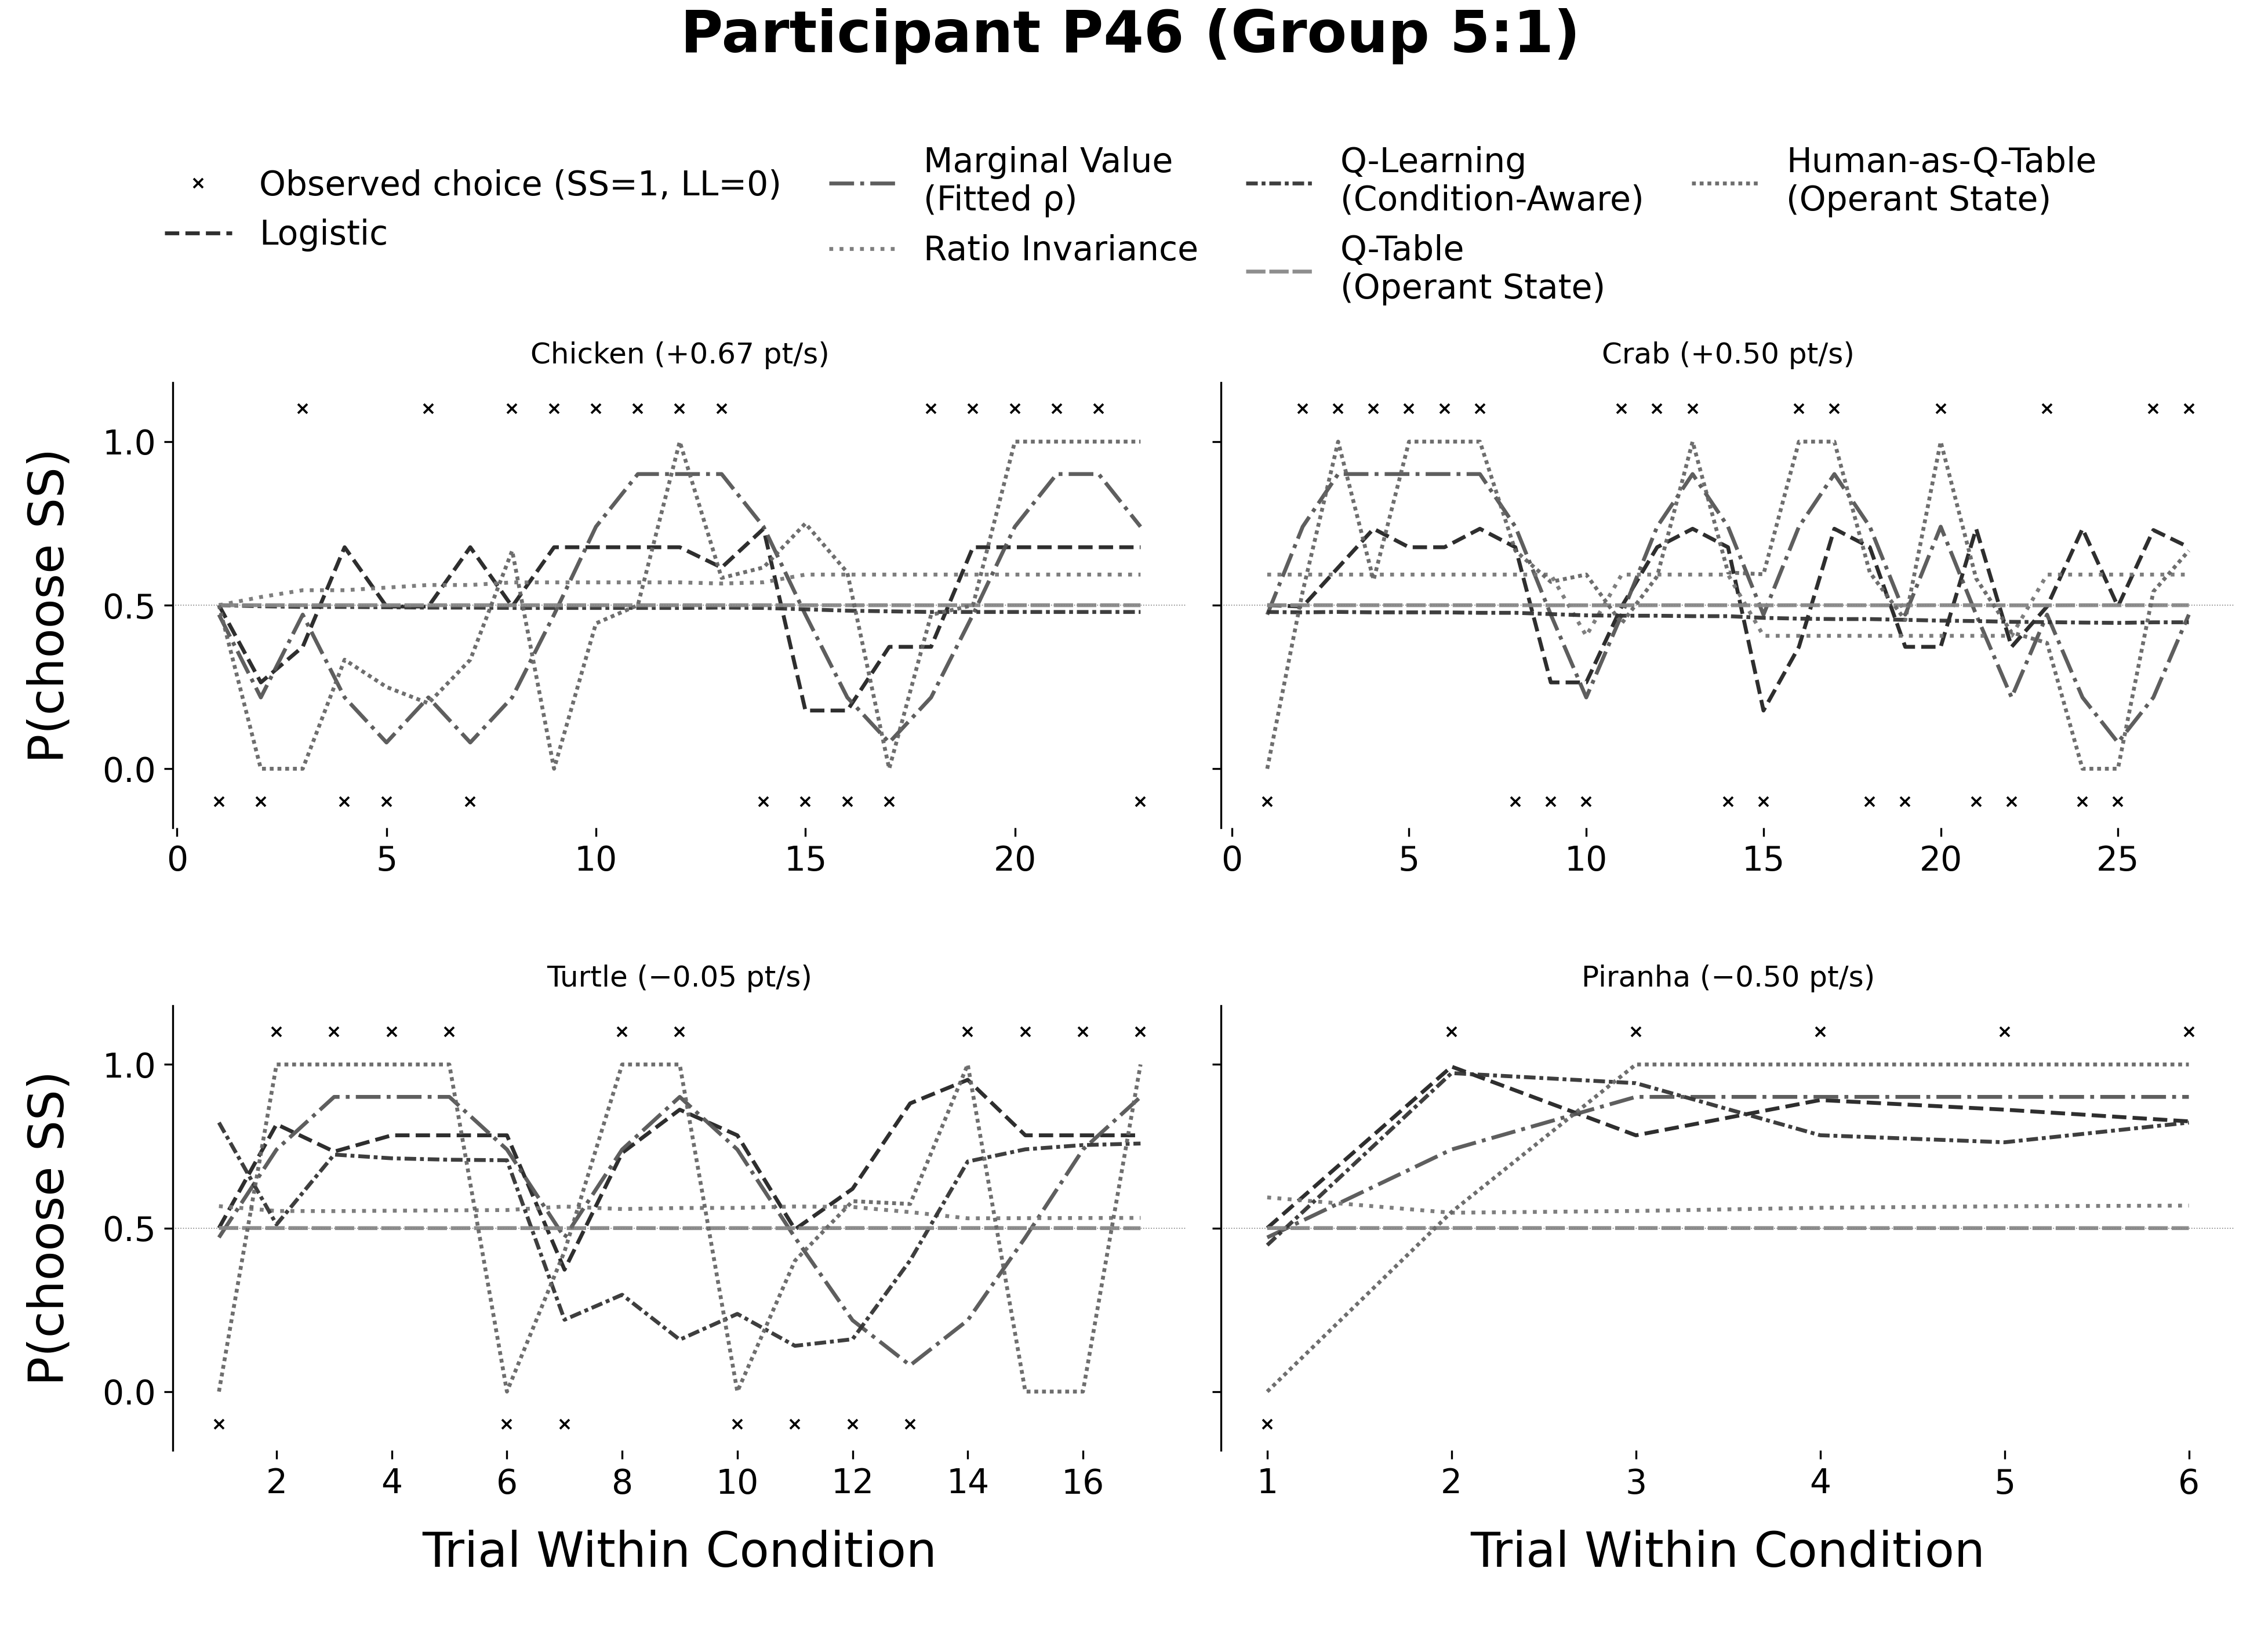
\includegraphics[width=\textwidth]{data/results/figures/appendix_b/fig_participant_Exp1_05_P46.png}
  \caption{Trial-by-trial model fit for participant Exp1\_05\_P46 (Group 5:1). Each panel is one earning-budget condition. Black x marks are the participant's raw choices (SS${}=1$, LL${}=0$), plotted just outside the $[0,1]$ band. Gray lines are the predicted $P(\mathrm{SS})$ of the best-fitting model in each family.}
\end{figure}

\begin{figure}[p]
  \centering
  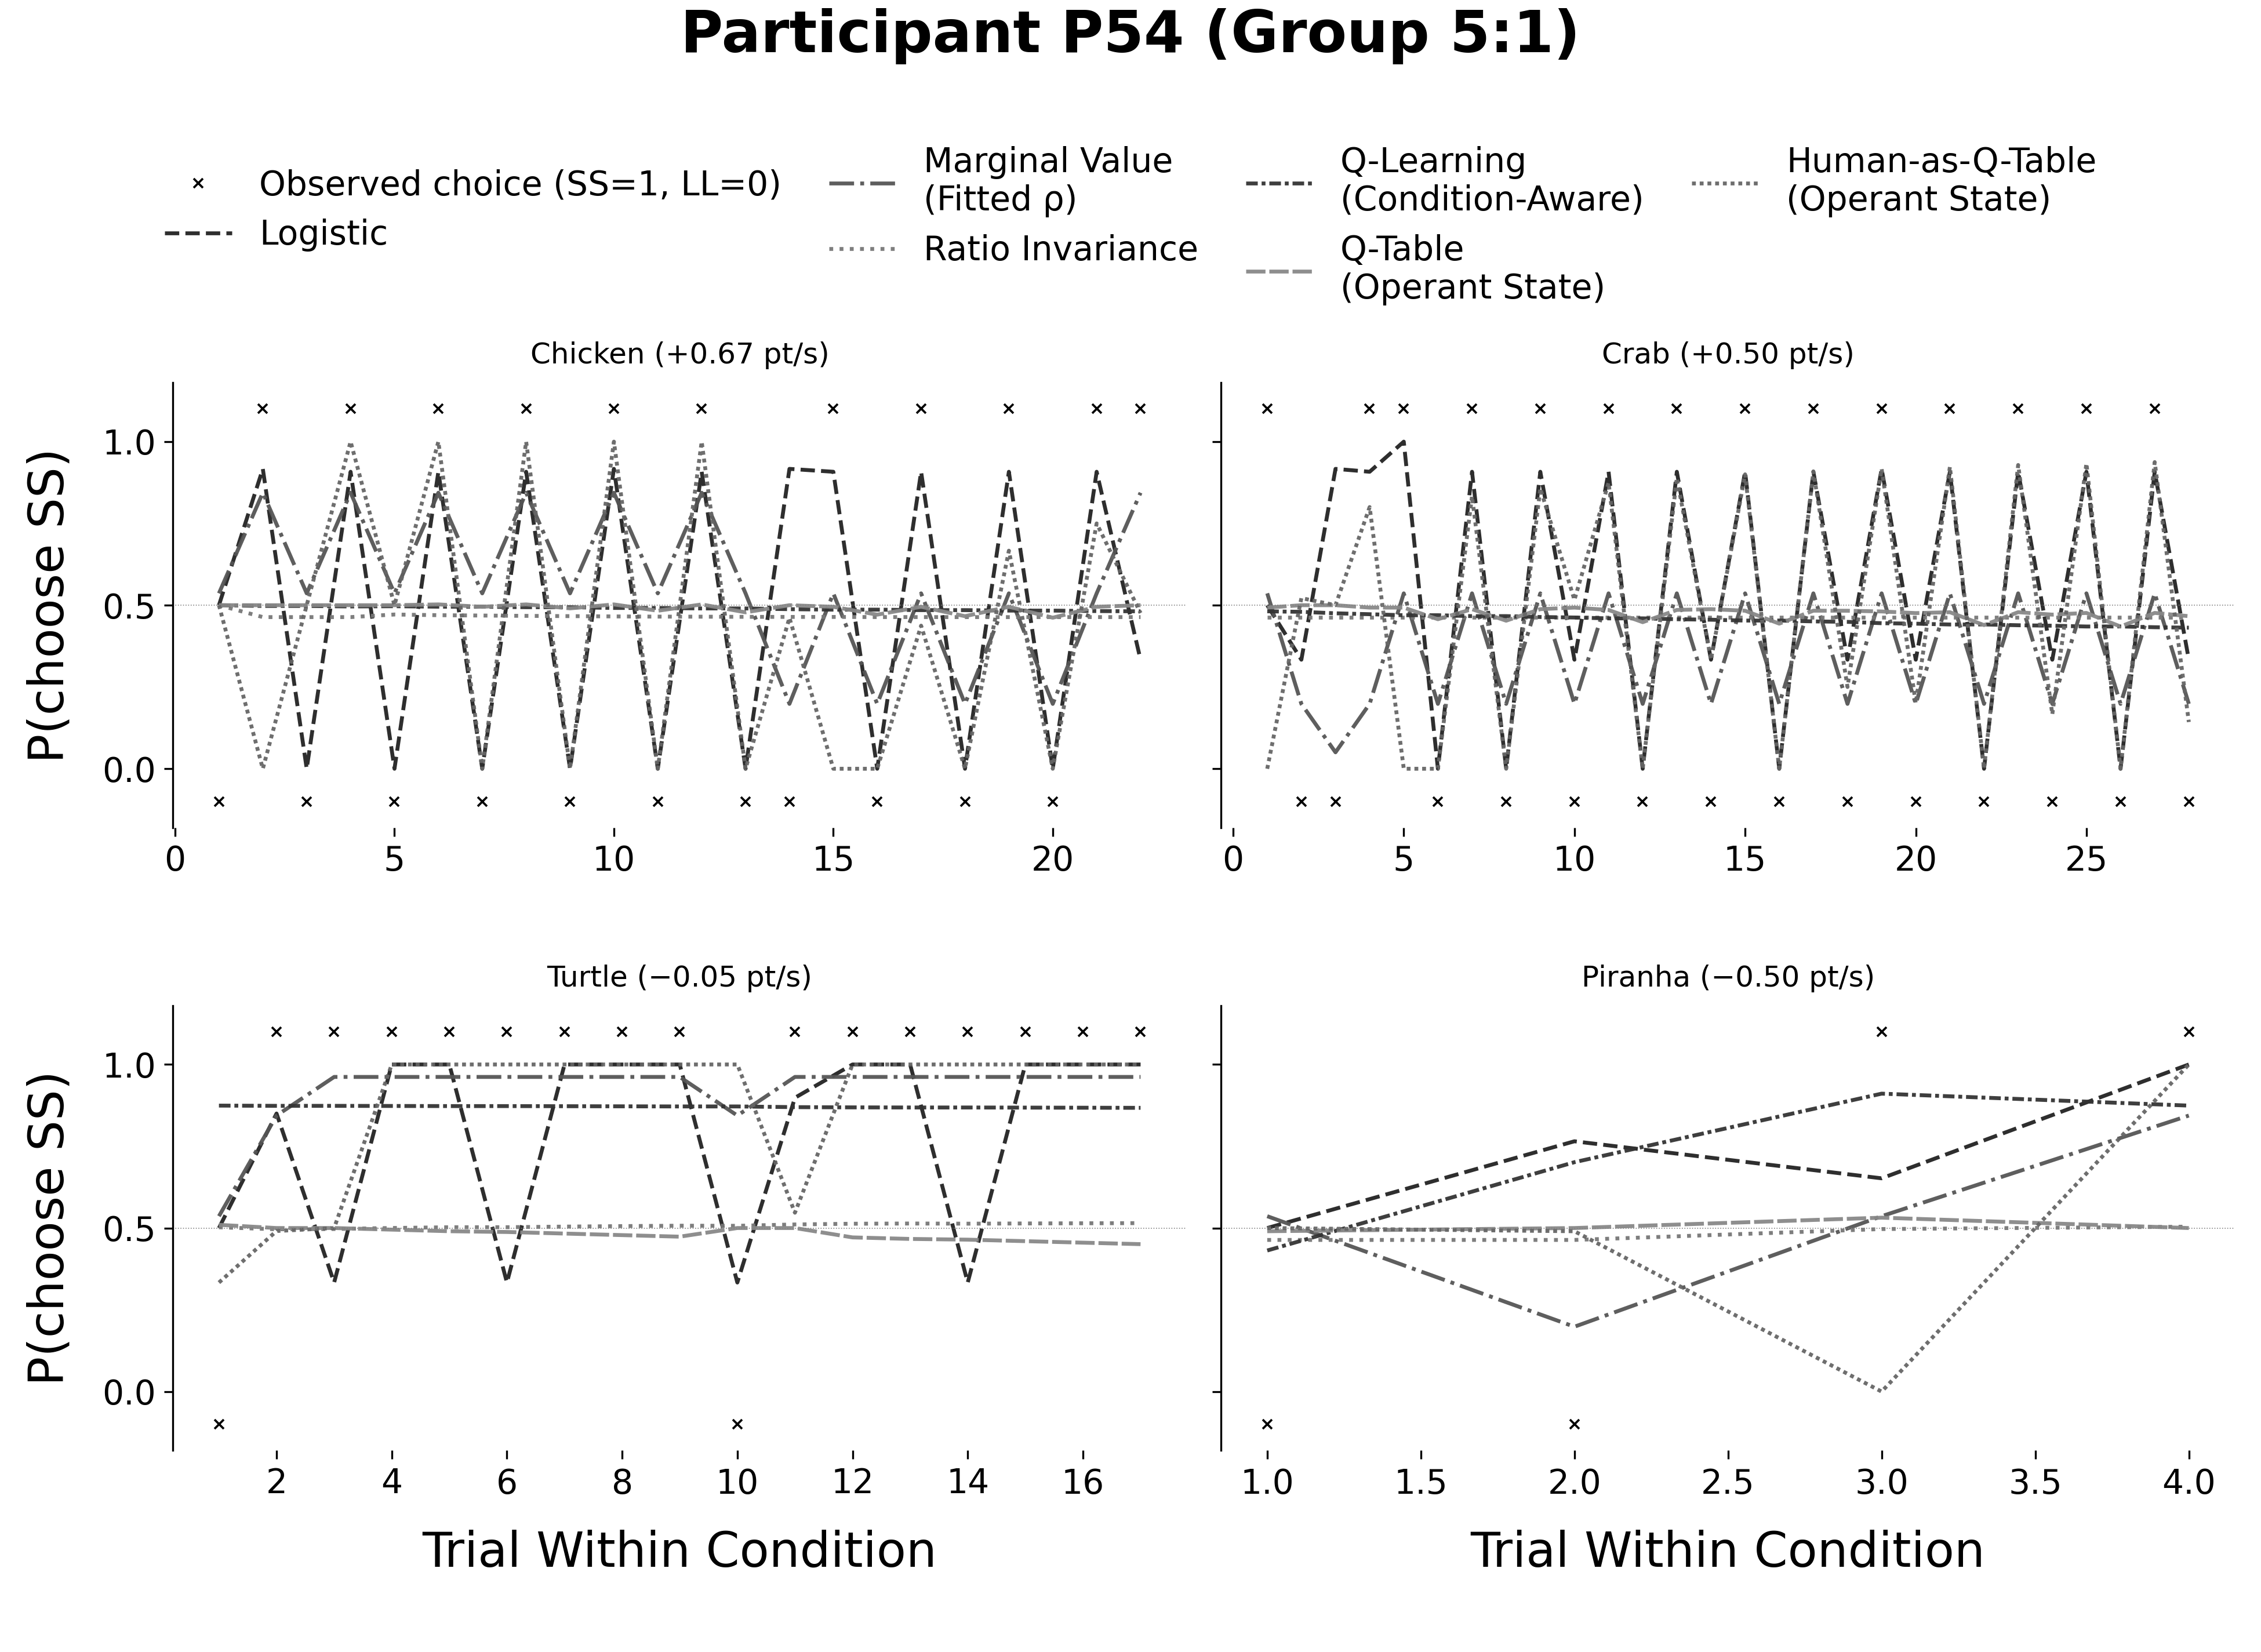
\includegraphics[width=\textwidth]{data/results/figures/appendix_b/fig_participant_Exp1_05_P54.png}
  \caption{Trial-by-trial model fit for participant Exp1\_05\_P54 (Group 5:1). Each panel is one earning-budget condition. Black x marks are the participant's raw choices (SS${}=1$, LL${}=0$), plotted just outside the $[0,1]$ band. Gray lines are the predicted $P(\mathrm{SS})$ of the best-fitting model in each family.}
\end{figure}

\begin{figure}[p]
  \centering
  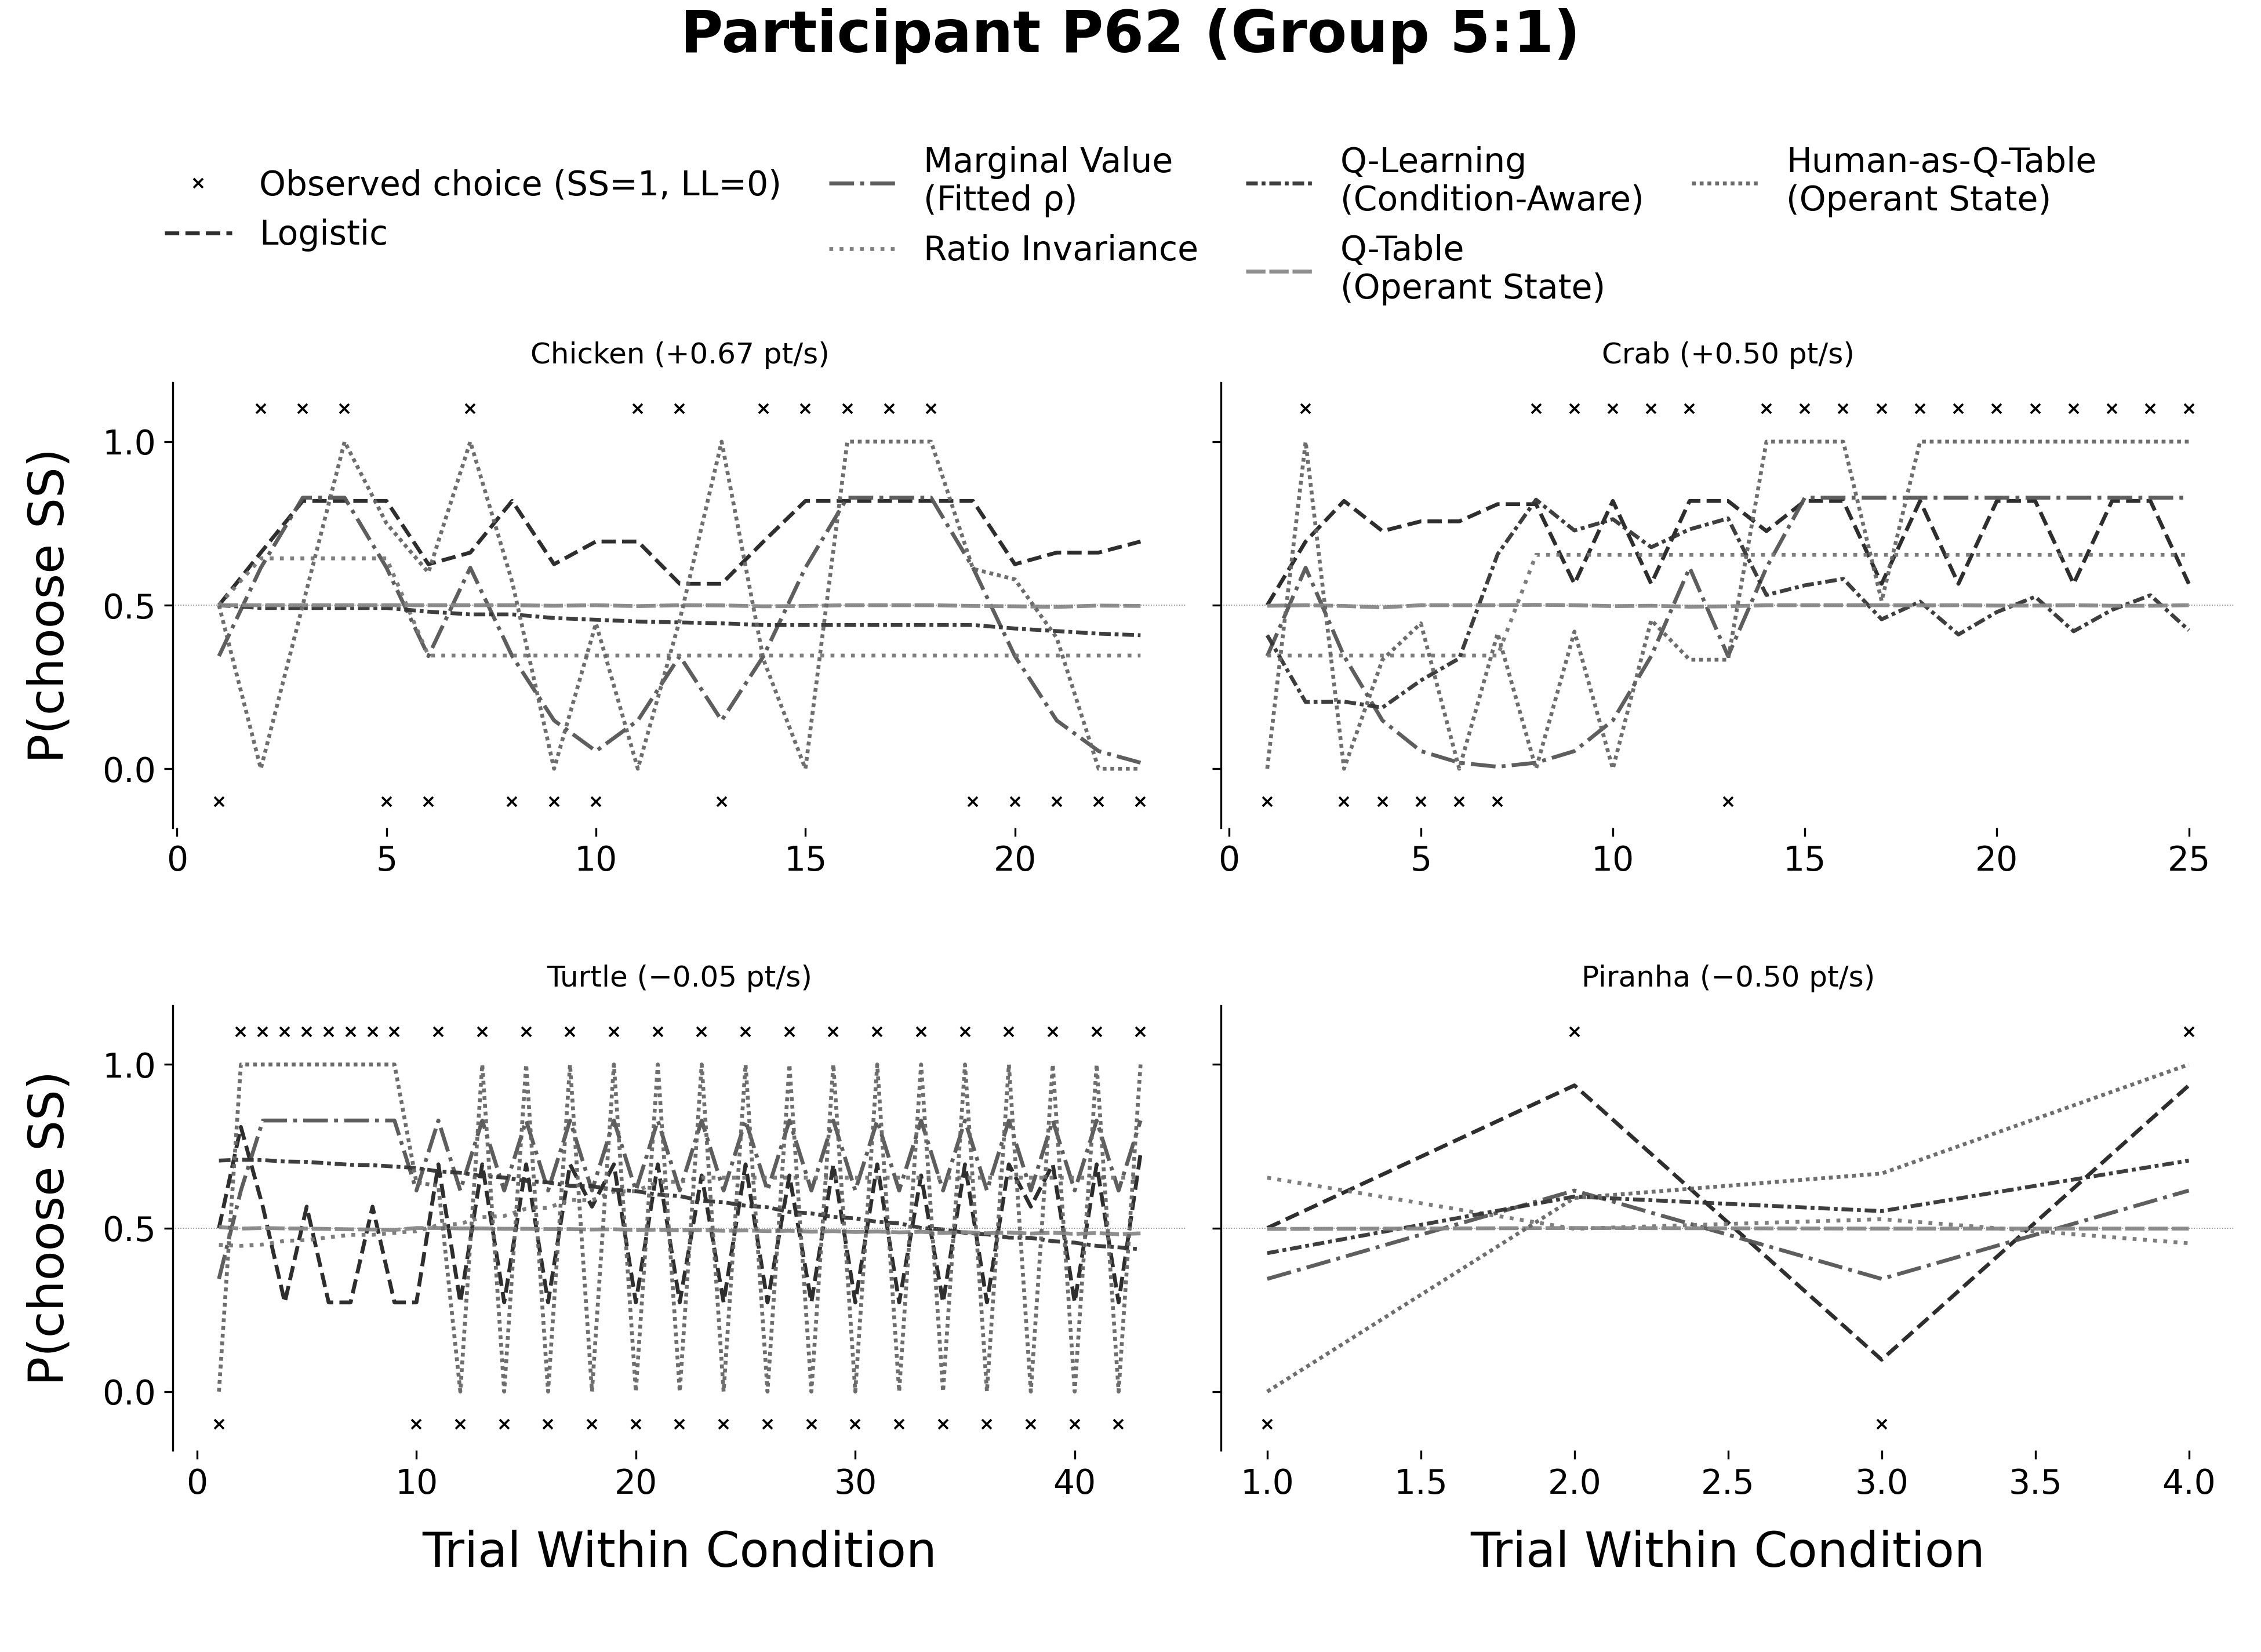
\includegraphics[width=\textwidth]{data/results/figures/appendix_b/fig_participant_Exp1_05_P62.png}
  \caption{Trial-by-trial model fit for participant Exp1\_05\_P62 (Group 5:1). Each panel is one earning-budget condition. Black x marks are the participant's raw choices (SS${}=1$, LL${}=0$), plotted just outside the $[0,1]$ band. Gray lines are the predicted $P(\mathrm{SS})$ of the best-fitting model in each family.}
\end{figure}

\begin{figure}[p]
  \centering
  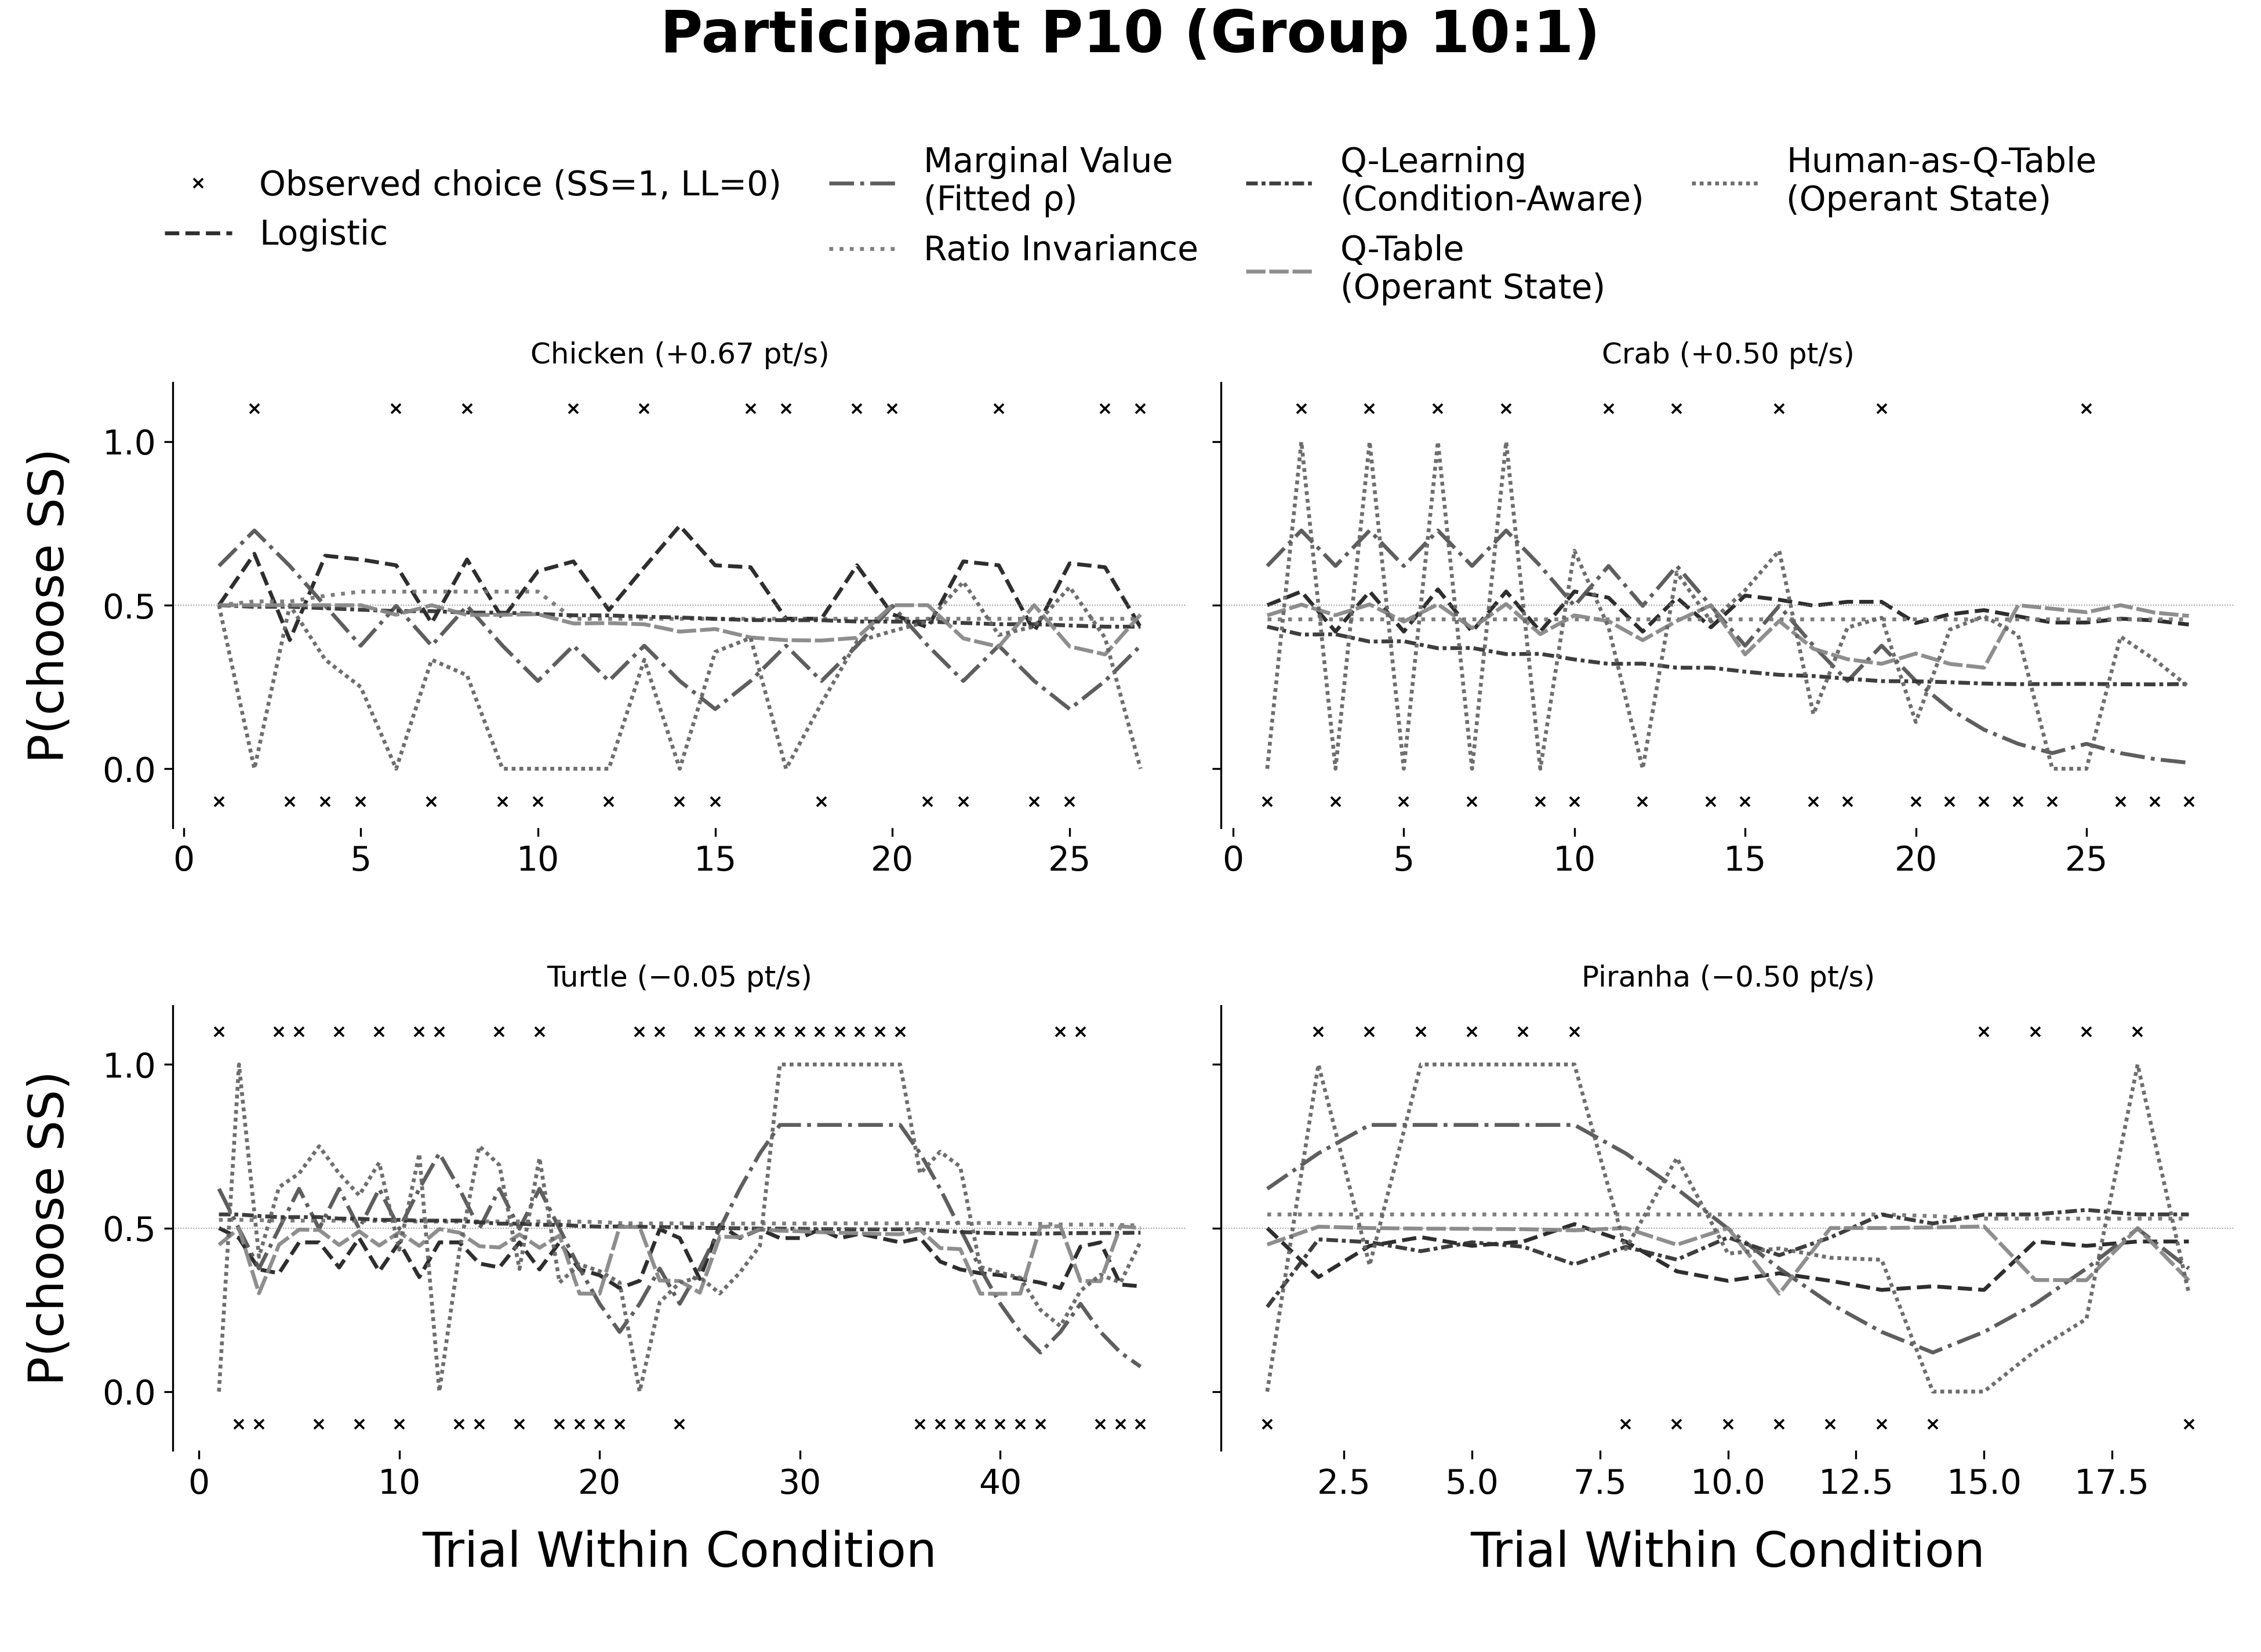
\includegraphics[width=\textwidth]{data/results/figures/appendix_b/fig_participant_Exp1_10_P10.png}
  \caption{Trial-by-trial model fit for participant Exp1\_10\_P10 (Group 10:1). Each panel is one earning-budget condition. Black x marks are the participant's raw choices (SS${}=1$, LL${}=0$), plotted just outside the $[0,1]$ band. Gray lines are the predicted $P(\mathrm{SS})$ of the best-fitting model in each family.}
\end{figure}

\begin{figure}[p]
  \centering
  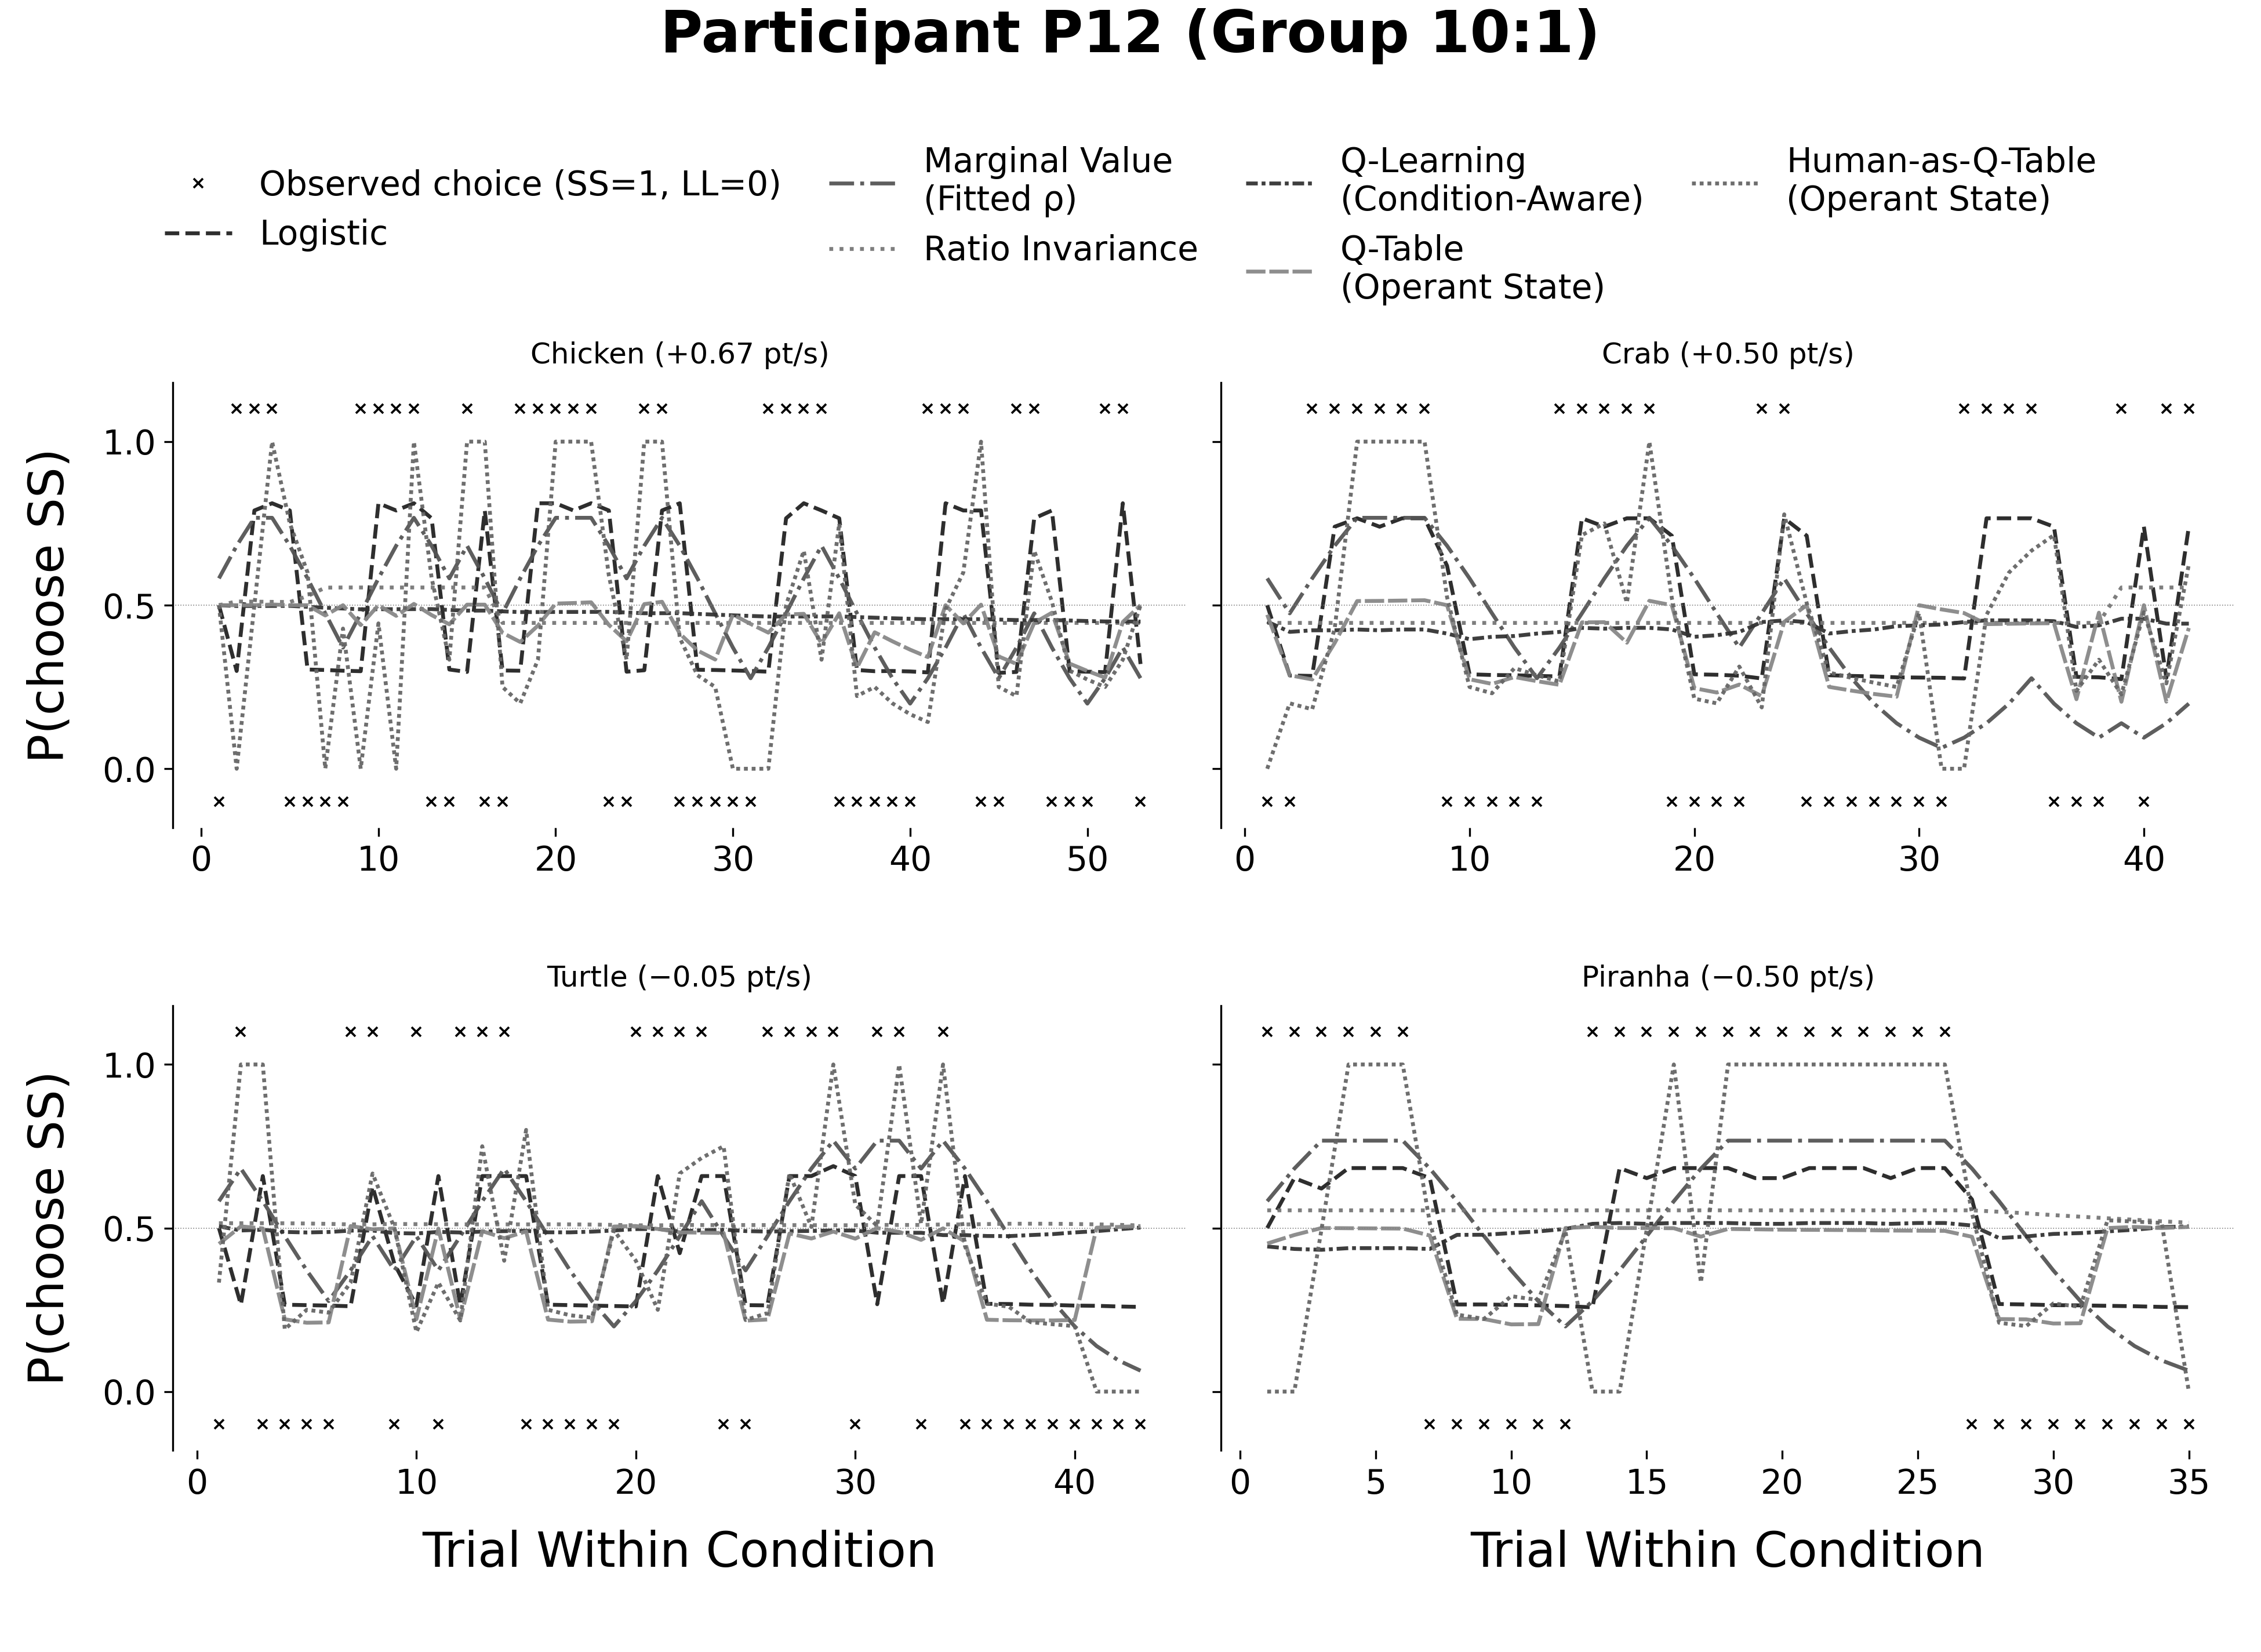
\includegraphics[width=\textwidth]{data/results/figures/appendix_b/fig_participant_Exp1_10_P12.png}
  \caption{Trial-by-trial model fit for participant Exp1\_10\_P12 (Group 10:1). Each panel is one earning-budget condition. Black x marks are the participant's raw choices (SS${}=1$, LL${}=0$), plotted just outside the $[0,1]$ band. Gray lines are the predicted $P(\mathrm{SS})$ of the best-fitting model in each family.}
\end{figure}

\begin{figure}[p]
  \centering
  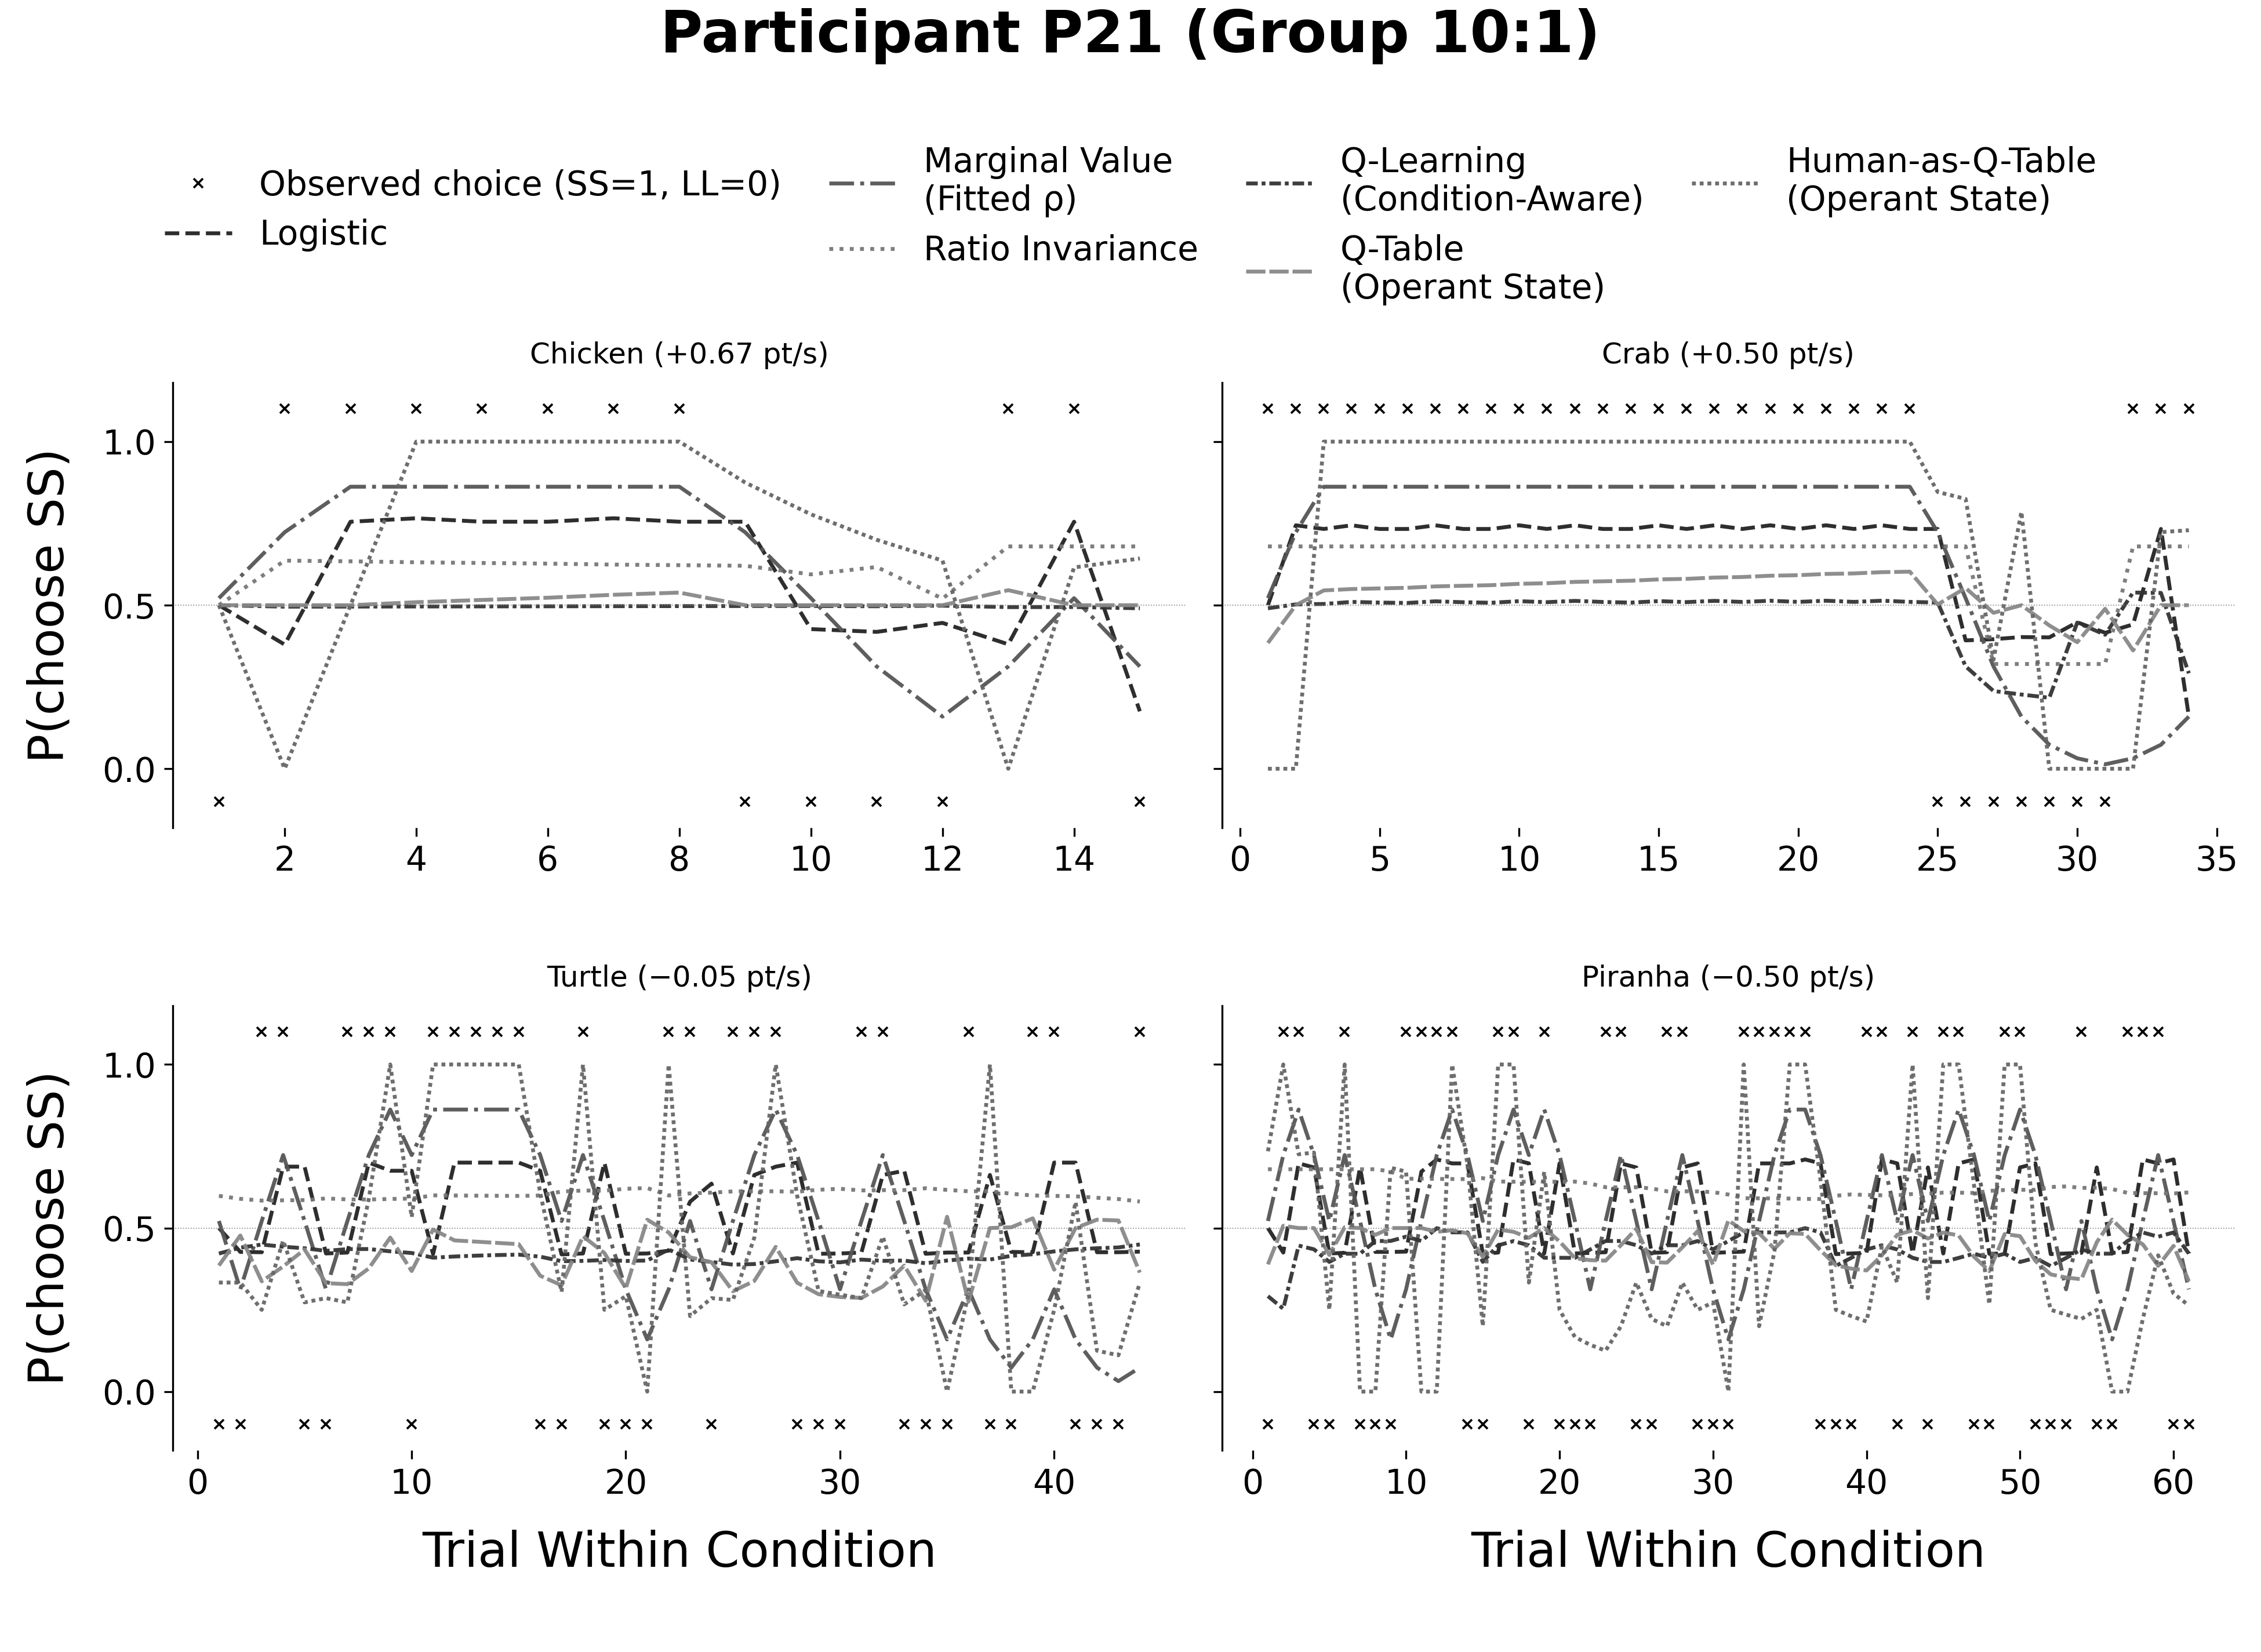
\includegraphics[width=\textwidth]{data/results/figures/appendix_b/fig_participant_Exp1_10_P21.png}
  \caption{Trial-by-trial model fit for participant Exp1\_10\_P21 (Group 10:1). Each panel is one earning-budget condition. Black x marks are the participant's raw choices (SS${}=1$, LL${}=0$), plotted just outside the $[0,1]$ band. Gray lines are the predicted $P(\mathrm{SS})$ of the best-fitting model in each family.}
\end{figure}

\begin{figure}[p]
  \centering
  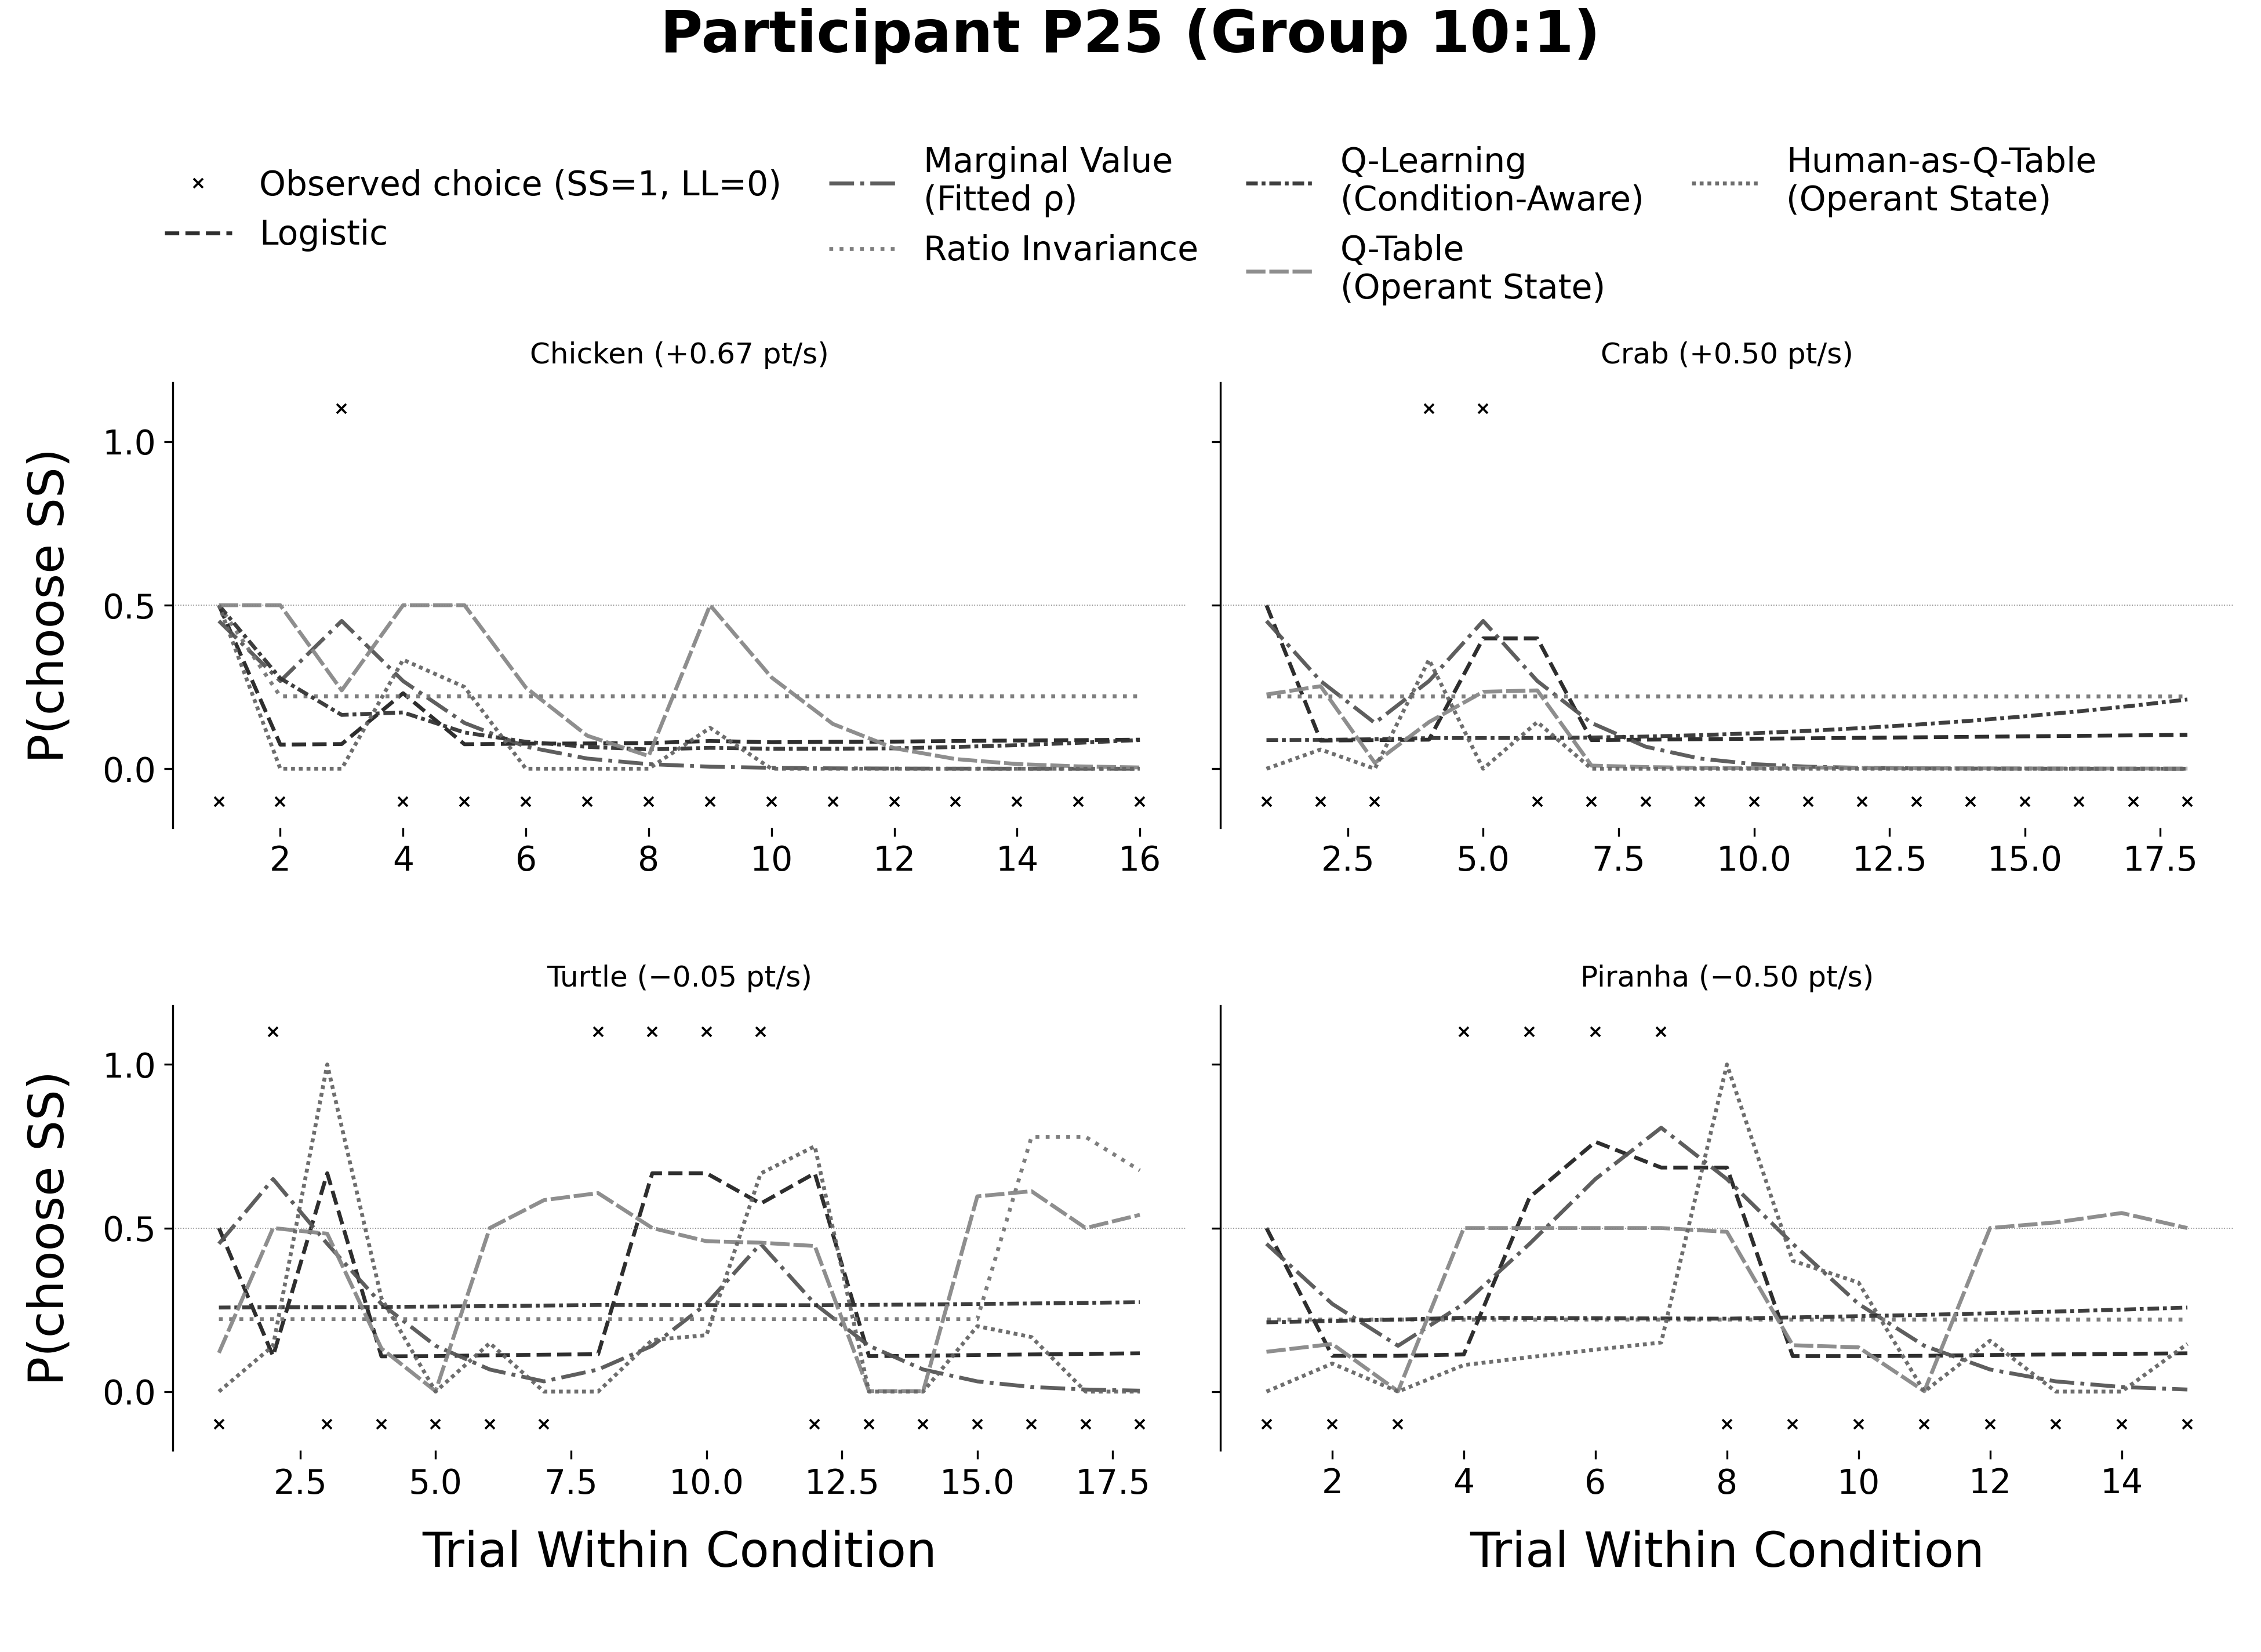
\includegraphics[width=\textwidth]{data/results/figures/appendix_b/fig_participant_Exp1_10_P25.png}
  \caption{Trial-by-trial model fit for participant Exp1\_10\_P25 (Group 10:1). Each panel is one earning-budget condition. Black x marks are the participant's raw choices (SS${}=1$, LL${}=0$), plotted just outside the $[0,1]$ band. Gray lines are the predicted $P(\mathrm{SS})$ of the best-fitting model in each family.}
\end{figure}


\end{document}
